\documentclass[12pt]{article}
\usepackage{graphicx}
\usepackage{longtable}
\usepackage{listings}
\usepackage[letterpaper, margin=2cm]{geometry}
\usepackage[T1]{fontenc}
\usepackage{polski}
\usepackage[export]{adjustbox}
\usepackage[utf8]{inputenc}
\usepackage[polish]{babel}
\graphicspath{{.}}
\usepackage{tocloft}
\usepackage{hyperref}

\hypersetup{%
    colorlinks,
    citecolor=black,
    filecolor=black,
    linkcolor=black,
    urlcolor=black
}

\renewcommand{\cftsecleader}{\cftdotfill{\cftdotsep}}

\lstset{
    postbreak=\mbox{\textcolor{red}{$\hookrightarrow$}\space}
    belowcaptionskip=1\baselineskip,
    breaklines=true,
    frame=L,
    numbers=left,
    xleftmargin=\parindent,
    language=bash,
    showstringspaces=false,
    basicstyle=\footnotesize\ttfamily,
    identifierstyle=\color{blue},
    stringstyle=\color{orange},
}

\begin{document}
    \centering
    
\includegraphics[width=5cm, height=5cm,]{herbPL.jpg}
    \hspace{2cm}
    
\includegraphics[width=5cm, height=5cm]{herbWEII.jpg}\\
    \vspace{2cm}
    {\Huge \textbf{SPRAWOZDANIE}}
    \vspace{2cm}
    \newline
    {\large PROGRAMOWANIE W CHMURZE OBLICZENIOWEJ}
    \vfill
    \raggedright
    \textbf{IMIĘ I NAZWISKO:} Piotr Czajka

    \textbf{NUMER LABORATORIUM} 3\\
    \textbf{GRUPA:} 7.1.2\\
    \textbf{Data wykonywania ćwiczenia:} 25.10.2018\\

    \newpage

    \tableofcontents{}

    \newpage

    \section{Cel laboratorium}
    Celem laboratorium było zapoznanie się z konfiguracją połączeń sieciowych i komunikacją w środowisko Docker\\

    \section{Przebieg ćwiczenia}

    \subsection{Zadanie pierwsze}

    Najpierw należało wykonać odpowiednią sieć. Robi to skrypt zamieszczony poniżej. Ponadto zawiera on komentarze w miejscach wartych zainteresowania:

    \lstinputlisting[language=bash]{ex1.sh}

    \subsubsection{Podpunkt pierwszy}

    W moim przypadku zmapowałem porty 8080 i 8081 do kontenera D2, ponieważ server Tomcat w tym kontenerze słuchał na porcie 80

    \subsubsection{Podpunkt drugi}

    Realizują go następujące linie:

    \lstinputlisting[language=bash, firstline=32, lastline=35]{ex1.sh}

    \subsubsection{Podpunkt trzeci}

    Tu chyba jest błąd w instrukcji. Kontener D1 został połączony z siecią ze zdefiniowanym subnetem, myślę, że chodziło raczej o kontener D2, który razem z kontenerem S1 został połączony z siecią bez filtrowania. A zrealizowały to następunące linie.

    Tu tworzę sieć:

    \lstinputlisting[firstline=23, lastline=23]{ex1.sh}

    Tu tworzę D2 i przyłączam go do tej sieci:

    \lstinputlisting[firstline=26, lastline=27]{ex1.sh}

    To samo dla S1:

    \lstinputlisting[firstline=24, lastline=24]{ex1.sh}

    Komunikację kontener -> host osiągam za pomovą modyfikacji na hoscie za pomocą tych poleceń:

    \lstinputlisting[firstline=1, lastline=2]{ex1.sh}

    Możliwość połączenia z kontenera do hosta potwierdza poniższy screen:

    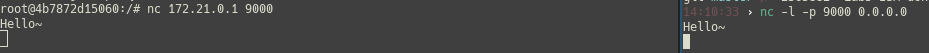
\includegraphics[width=\textwidth]{pic1.png}

    \subsubsection{Konfiguracje sieci}

    Sieć domyślna:

    \lstinputlisting{net1.txt}

    \vspace{0.5cm}

    Jak widać tu:

    \lstinputlisting[firstline=27, lastline=41]{net1.txt}

    Do sieci tej zostały podłączone kontenery T1 i T2

    \vspace{2cm}

    Sieć bridge1:

    \lstinputlisting{net2.txt}

    \vspace{0.5cm}

    Hosty D1, D2, T2, late połączone z tą siecią, wszystkie mają IP z subnetu 10.0.10.0:

    \lstinputlisting[firstline=26, lastline=54]{net2.txt}

    Część mówiąca o subnet jest tu:

    \lstinputlisting[firstline=12, lastline=16]{net2.txt}

    \vspace{2cm}

    I sieć bridge2:

    \lstinputlisting{net3.txt}
    \vspace{0.5cm}

    Połączone hosty:

    \lstinputlisting[firstline=25, lastline=54]{net2.txt}

    \vspace{0.5 cm}

    Został przydzielony do niej taki oto subnet i brama domyślna za pomocą której możemy komunikować się z komputerem hosta:

    \lstinputlisting[firstline=12, lastline=17]{net2.txt}

    \vspace{2cm}

    Tablica routingu T2:

    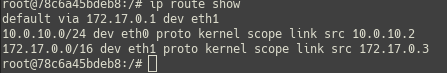
\includegraphics[width=\textwidth]{T2route.png}

    \vspace{0.5cm}

    Tablica routingu D2:

    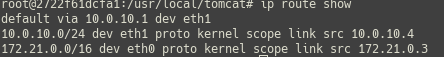
\includegraphics[width=\textwidth]{D2route.png}

    \subsubsection{Pytanie pierwsze:}

    Poniższy screen przedstawia, jak komunikat 'Hello' poprawnie został przesłany z kontenera D2 na host posługując się programem 'netcat'. Komunikacja przebiegała przez port 9000:

    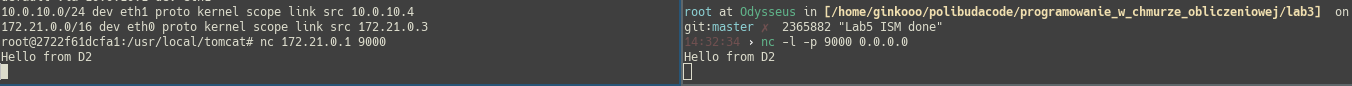
\includegraphics[width=\textwidth]{D2hello.png}

    To samo dla S1 -> host:

    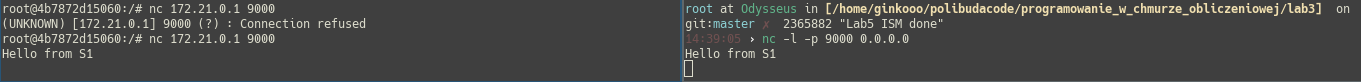
\includegraphics[width=\textwidth]{S1hello.png}

    \vspace{1cm}

    {\large Podpunkt a:}
    \vspace{0.5cm}

    Możliwym jest przekazanie parametru '--ip-range' przy poleceniu 'docker network create'. Np '--ip-range=172.28.5.0/24'


    \subsection{Zadanie drugie}

    Po uruchomieniu zalinkowanych kontenerów zawartość zmiennych systemowych w T1 prezentuje się tak:

    \lstinputlisting{envT1.txt}

    Te zmienne używane są przez kod linkujący:

    \lstinputlisting[firstline=20, lastline=31]{envT1.txt}

    A tak prezentuje się plik '/etc/hosts'

    \lstinputlisting{hostsT1.txt}

    Linker oczywiście używa wpisu z 7. linijce.

    \subsubsection{Pytanie pierwsze}

    Ping z maszyny T1 na T2 jest możliwy, T1 ma też odpowiedni wpis w 'hosts'. Natomiast ping z T2 na T1 konczy się niepowodzeniem. Tam też nie ma wpisu w '/etc/hosts' wskazującego naa kontener T1. Potwierdza to poniższy zrzut ekranu:

    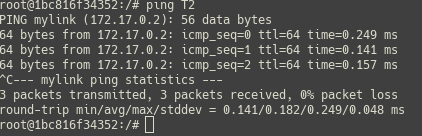
\includegraphics[width=\textwidth]{pingt1t2.png}

    \subsubsection{Pytanie drugie}

    {\Large Tryb sieci host:}

    Docker odmawia utworzenia kontenera z linkiem do innego kontenera. W tym trybie kontener korzysta z natywnego stosu sieciowego hosta, a nie z oddzielnych sieci, nie ma więc czego linkować ze sobą.

    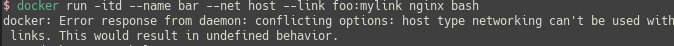
\includegraphics[width=\textwidth]{hostlink.png}

    \vspace{0.5cm}

    {\Large User definied bridge:}

    Polecenie tworzenia linków działa bez zarzutów. Jest ono jednak zbędne, bo w tym trybie urządzenia i tak widzą się całkowicie, potwierdza to ping z foo na bar:

    \vspace{0.2cm}

    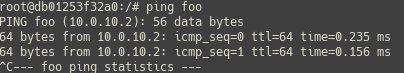
\includegraphics[width=\textwidth]{foobrping.png}

    Plik hosts w foo:

    \vspace{0.2cm}
    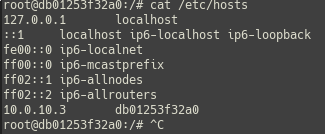
\includegraphics[width=\textwidth]{foobrhosts.png}

    I hosts w bar:

    \vspace{0.2cm}
    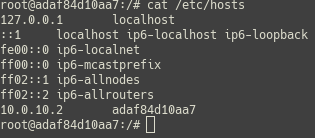
\includegraphics[width=\textwidth]{barbrhosts.png}

    \subsubsection{Pytanie trzecie:}

    Utworzyłem kontener 'bar' w domyślnej sieci i 'foo' w sieci user-defined-brige. Po stworzeniu foo z linkiem do bar plik '/etc/hosts' w 'foo' nie posiada wymaganych wpisów:

    \vspace{0.2cm}

    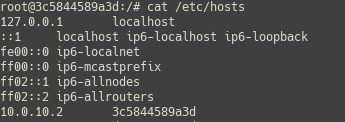
\includegraphics[width=\textwidth]{hostsfail.png}

    Ping foo -> bar też nie działa.

    \vspace{0.2cm}

    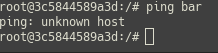
\includegraphics[width=\textwidth]{pingfail.png}

    Próba stworzenia linku w trybie sieci host kończy się takim samym błędem jak wcześniej. Wniosek - nie da się.

    \subsection{Zadanie trzecie:}

    Skrypt zmodyfikowany o użycie aliasów:

    \lstinputlisting[language=bash]{ex3.sh}

    \subsubsection{Pytanie pierwsze:}

    Nie, taka komunikacja nie jest możliwa, co widać na poniższym screenie, ping host2 -> host1 się nie powiódł.

    \vspace{0.2cm}

    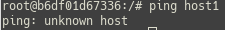
\includegraphics[width=\textwidth]{aliaspingfail.png}

    Takie aliasy działają tylko w obrębie tej samej sieci. Linux udostępnia konsktukt zwany "network namespace", który umożliwia oddzielenie od siebie logicznych fragmentów sieci i zdefiniowanie dla nich zupełnie niezależnych regół, aliasów itd., z czego korzysta też Docker.

    \subsubsection{Pytanie drugie:}

    Aby korzystać z tych aliasów trzeba by zmodyfikować '/etc/hosts' na komputerze macierzystym, czego Docker nie robi podczas tworzenia tych kontenerów, możliwym też by była translacja nazw za pomocą pośredniego serwera DNS, co nie zostało skonfigurowane. Więc - domyślnie nie jest to możliwe od razu.

\end{document}
